% \iffalse
\let\negmedspace\undefined
\let\negthickspace\undefined
\documentclass[article]{IEEEtran}
\usepackage{float}
\usepackage{circuitikz}
\usepackage{cite}
\usepackage{amsmath,amssymb,amsfonts,amsthm}
\usepackage{algorithmic}
\usepackage{graphicx}
\usepackage{textcomp}
\usepackage{xcolor}
\usepackage{txfonts}
\usepackage{listings}
\usepackage{amsmath}
\usepackage{enumitem}
\usepackage{mathtools}
\usepackage{gensymb}
\usepackage{comment}
\usepackage[breaklinks=true]{hyperref}
\usepackage{tkz-euclide} 
\usepackage{listings}
\usepackage{gvv}                                        
\def\inputGnumericTable{}                                 
\usepackage[latin1]{inputenc}                               \usepackage{} 
\usepackage{color}                                            
\usepackage{array}                                            
\usepackage{longtable}                                       
\usepackage{calc}  
\usepackage{caption}
\usepackage{multirow}                                         
\usepackage{hhline}                                           
\usepackage{ifthen}                                           
\usepackage{lscape}
\newtheorem{theorem}{Theorem}[section]
\newtheorem{problem}{Problem}
\newtheorem{proposition}{Proposition}[section]
\newtheorem{lemma}{Lemma}[section]
\newtheorem{corollary}[theorem]{Corollary}
\newtheorem{example}{Example}[section]
\newtheorem{definition}[problem]{Definition}
\newcommand{\BEQA}{\begin{eqnarray}}
\newcommand{\EEQA}{\end{eqnarray}}
\newcommand{\define}{\stackrel{\triangle}{=}}
\theoremstyle{remark}
\newtheorem{rem}{Remark}
\renewcommand\thesection{\arabic{section}}
\renewcommand\thesubsection{\thesection.\arabic{subsection}}
\renewcommand\thesubsubsection{\thesubsection.\arabic{subsubsection}}

\renewcommand\thesectiondis{\arabic{section}}
\renewcommand\thesubsectiondis{\thesectiondis.\arabic{subsection}}
\renewcommand\thesubsubsectiondis{\thesubsectiondis.\arabic{subsubsection}}
\lstset{
language=Python,
frame=single, 
breaklines=true,
columns=fullflexible
}
\numberwithin{equation}{subsection}
\renewcommand{\thesubsection}{\thesection.\arabic{subsection}}
\makeatletter
\renewcommand\section{\@startsection {section}{1}{\z@}%
    {-3.5ex \@plus -1ex \@minus -.2ex}%
    {2.3ex \@plus.2ex}%
    {\normalfont\large\bfseries}}
\renewcommand\subsection{\@startsection{subsection}{2}{\z@}%
    {-3.25ex\@plus -1ex \@minus -.2ex}%
    {1.5ex \@plus .2ex}%
    {\normalfont\large\bfseries}}
\makeatother
\usepackage{tcolorbox}

% Define a command for highlighting equations
\newcommand{\highlighteq}[1]{%
    \begin{tcolorbox}[colback=blue!5!white,colframe=blue!75!black,title=Highlighted Equation]
    #1
    \end{tcolorbox}%
}
\begin{document}

\bibliographystyle{IEEEtran}
\vspace{3cm}
\title{Filter Design \#1}
\author{EE23BTECH11013 -  Avyaaz
}
\maketitle
% \newpage
% \bigskip
\renewcommand{\thefigure}{\arabic{figure}}
\renewcommand{\thetable}{\arabic{figure}}

\bibliographystyle{IEEEtran}

 % \tableofcontents

\maketitle
%-------------------------------------------------------------------------------
\section{\textbf{Introduction}}
We are supposed to design the equivalent FIR and IIR filter realizations for filter number 1. 
The filter numbers are calculated using the below code:
\begin{lstlisting}
    wget avk
\end{lstlisting}
This is a bandpass filter whose specifications are available below.

\section{\textbf{Filter Specifications}}
The sampling rate for the filter has been specified as $F_s =  48$ kHz.	If the un-normalized  discrete-time (natural) frequency is F, the corresponding normalized digital filter (angular) frequency is given by $\omega = 2\pi
\left(\frac{F}{F_s}\right)$.

\subsection{\textbf{The Digital Filter}}
\begin{enumerate}[label = \roman*)]
    \item \textit{Tolerances:} The passband ($\delta_1$) and stopband ($\delta_2$) tolerances are given to be equal, so we let $\delta_1 = \delta_2 = \delta = 0.15$.
    
    \item \textit{Passband:} The passband of filter number $j$, $j$ going from 0 to 13 is from \{4 + 0.6$j$\}kHz to \{4 + 0.6$(j + 2)$\}kHz. Since our filter number is 1, substituting $j = 1$ gives the passband range for our bandpass filter as $4.6$ kHz - $5.8$ kHz. Hence, the un-normalized discrete time filter passband frequencies are:
    \begin{align}
        F_{p_1} = 5.8 \text{ kHz}\\
        F_{p_2} = 4.6 \text{ kHz}
    \end{align} The corresponding normalized digital filter passband frequencies are:
    \begin{align}
        \omega_{p_1} = 2\pi\frac{F_{p_1}}{F_s}  = 0.2416\pi\text{ kHz}\\
        \omega_{p_2} = 2\pi\frac{F_{p_2}}{F_s}  = 0.1916 \pi \text{ kHz}
    \end{align} The centre frequency is then given by:
    \begin{align}
        \omega_c = \frac{\omega_{p_1} + \omega_{p_2}}{2} = 0.2166\pi
    \end{align}  
    
    \item \textit{Stopband:} The \textit{transition band} for bandpass filters is $\Delta F = 0.3$ kHz on either side of the passband. Hence, the un-normalized \textit{stopband} frequencies are $F_{s_1} = 5.8 + 0.3 = 6.1$ kHz and $F_{s_2} = 4.6 - 0.3 = 4.3$ kHz. The corresponding normalized frequencies are $\omega_{s_1} = 0.25416 \pi$ and $\omega_{s_2} = 0.17916 \pi$.
\end{enumerate}
\subsection{The Analog filter}
In the bilinear transform, the analog filter frequency ($\Omega$) is related to the corresponding digital filter frequency ($\omega$) as:
\begin{align}
    \Omega = \tan \frac{\omega}{2}
\end{align} Using this relation, we obtain the analog passband and stopband frequencies as $\Omega_{p_1} = 0.399$, $\Omega_{p_2} = 0.311$ and $\Omega_{s_1} = 0.422$, $\Omega_{s_2} = 0.289$
respectively.

\section{The IIR Filter Design}
{\em Filter Type:}  We are supposed to design filters whose stopband is monotonic and passband equiripple.  
Hence, we use the {\em Chebyschev approximation} to design our bandpass IIR filter.

\subsection{The Analog Filter}
\begin{enumerate}

\item {\em Low Pass Filter Specifications:}  If $H_{a, BP}(j\Omega)$ be the desired analog band
pass filter,  with the specifications provided in Section 2.2, and $H_{a,LP}(j\Omega_L)$ 
be the equivalent low pass filter, then
\begin{equation}
\label{transition}
\Omega_L = \frac{\Omega^2 - \Omega_0^2}{B\Omega}
\end{equation}

%\begin{equation}
%H_{a, BP}(j\Omega) =  H_{a,LP}(j\Omega_L) \vert_{ \Omega_L = 
%\frac{\Omega^2 - \Omega_0^2}{B\Omega}},
%\end{equation}
where,

$\Omega_0 = \sqrt{\Omega_{p1}\Omega_{p2}} = 0.352$ and $B = \Omega_{p1} - \Omega_{p2} = 0.088$.  The low pass filter has
the passband edge at $\Omega_{Lp} = 1$ and stopband edges at $\Omega_{Ls_1} = 1.459$ and $\Omega_{Ls_2} = -1.588$.  We choose the stopband edge of the analog low pass filter as $\Omega_{Ls} = \mbox{min}(\vert \Omega_{Ls_1}\vert,\vert \Omega_{Ls_2}\vert) = 1.459$.

\item {\em The Low Pass Chebyschev Filter Paramters:}  The magnitude squared of the Chebyschev low pass filter is given by 
\begin{equation}
\label{lpfirst}
\vert H_{a,LP}(j\Omega_L)\vert^2 = \frac{1}{1 + \epsilon^2c_N^2(\Omega_L/\Omega_{Lp})}
\end{equation}
where $c_N(x) = \cosh(N \cosh^{-1}x)$ and the integer $N$, which is the order of the filter, and $\epsilon$ are design paramters.  Since $\Omega_{Lp} = 1$, (\ref{lpfirst}) may be rewritten as
\begin{equation}
\label{lpsecond}
\vert H_{a,LP}(j\Omega_L)\vert^2 = \frac{1}{1 + \epsilon^2c_N^2(\Omega_L)}
\end{equation}
Also, the design paramters have the following constraints
\begin{eqnarray}
\label{lpdesign}
\frac{\sqrt{D_2}}{c_N(\Omega_{Ls})} \leq \epsilon \leq \sqrt{D_1}, \nonumber \\
N \geq \left\lceil \frac{\cosh^{-1}\sqrt{D_2/D_1}}{\cosh^{-1}\Omega_{Ls}} \right\rceil,
\end{eqnarray}
where $D_1 = \frac{1}{(1 - \delta)^2}-1$ and $D_2 = \frac{1}{\delta^2} - 1$.  After appropriate substitutions,
we obtain:
\begin{align}
    &0.337 \leq \epsilon \leq 0.6197\\
    &N \geq 4 \\
    &D_1 = 0.3841\\
    &D_2 = 43.444
\end{align}
  In Figure 1, we plot $\vert H(j\Omega)\vert$ for a range of values of $\epsilon$, for $N = 4$. We find that for larger values of $\epsilon$, $|H(j\Omega)|$ decreases in the transition band.  We choose $\epsilon = 0.4$  for our IIR filter design.  

%For this value of $epsilon$, the plot of $\vert H(j\Omega) \vert$ is shown for various $4 \leq N \leq 10$.  For increasing values of $N$, we find that that fall from the passband to the stopband is sharp.  For $N = 6$, we find that $\vert H(j\Omega_{Ls}) \vert$ is very close to $\delta$, thus meeting the constraints imposed on the magnitude response of the filter.  Based on the above discussion, we choose $N = 6, \epsilon = 0.5$ as the design paramters for the equivalent lowpass Chebyschev approximation.  

\item {\em The Low Pass Chebyschev Filter:} Thus, we obtain
\begin{equation}
\label{lpsqfinal}
\vert H_{a,LP}(j\Omega_L)\vert^2 = \frac{1}{1 + 0.16c_4^2(\Omega_L)}
\end{equation}
where
\begin{equation}
c_4(x) = 8x^4 - 8x^2 + 1.	
\end{equation}
The poles of the frequency response in (\ref{lpfirst}) lying in the left half plane are in general obtained as 
$r_1\cos\phi_k + jr_2\sin \phi_k$, where
\begin{eqnarray}
\label{lppoles}
\phi_k = \frac{\pi}{2} + \frac{(2k+1)\pi}{2N}, k = 0, 1, \dots, N-1 \nonumber \\
r_1 = \frac{\beta^2 - 1}{2\beta}, r_2 = \frac{\beta^2 + 1}{2\beta}, \beta = \left[ \frac{\sqrt{1 + \epsilon^2} + 1}{\epsilon}\right]^{\frac{1}{N}}
\end{eqnarray}
Thus, for N even, the low-pass stable Chebyschev filter, with a gain $G$ has the form
\begin{equation}
\label{poleleft}
H_{a,LP}(s_L) = \frac{G_{LP}}{\prod_{k = 0}^{\frac{N}{2}-1}(s_L^2 - 2r_1\cos\phi_ks_L + r_1^2\cos^2\phi_k + r_2^2 \sin^2\phi_k)}
\end{equation}
Substituting $N = 4$, $\epsilon = 0.4$ and $H_{a,LP}(j) = \frac{1}{\sqrt{1+\epsilon^2}}$, from (\ref{lppoles}) and (\ref{poleleft}), we obtain 
\begin{equation}
\label{lpfinal}
H_{a,LP}(s_L) = \frac{0.3125}{s_L^4 + 1.1068s_L^3 + 1.6125s_L^2+0.9140s_L + 0.3366}
\end{equation}

In \figref{fig2} we plot $|H(j\Omega)|$ using (\ref{lpsqfinal}) and (\ref{lpfinal}), thereby verifying that our low-pass Chebyschev filter design meets the specifications.
\item {\em The Band Pass Chebyschev Filter:}  The analog bandpass filter is obtained from (\ref{lpfinal}) by substituting
$s_L = \frac{s^2 + \Omega_0^2}{Bs}$.  Hence
\begin{equation}
H_{a,BP}(s) = G_{BP}H_{a,LP}(s_L)\vert_{s_L = \frac{s^2 + \Omega_0^2}{Bs}},
\end{equation}
where $G_{BP}$ is the gain of the bandpass filter.  After appropriate substitutions, and evaluating the gain 
such that $H_{a,BP}(j\Omega_{p1}) = 1$, we obtain
{\tiny
\begin{align}
\label{bpfinal}
H_{a,BP}(s) &= \frac{2.0601\times 10^{-5}s^4}{s^8+0.0979s^7+0.5081s^6+0.0370s^5+0.0952s^4+0.0046s^3+0.0078s^2+0.0002s+0.0002}\\
G_{BP} & = 2.0601\times 10^{-5}
\end{align}
}
In Figure 3, we plot $\vert H_{a,BP}(j\Omega)\vert$ as a function of $\Omega$ for both positve as
well as negative frequencies.  We find that the passband and stopband frequencies in the figure
match well with those obtained analytically through the bilinear transformation.
\end{enumerate}

\begin{figure}[!ht]
\centering
\includegraphics[width = \columnwidth]{Figur1.png}
\caption{The Analog Low-Pass Frequency Response for $0.35 \leq \epsilon \leq 0.6$}
\label{fig1}
\end{figure}

\begin{figure}[!ht]
\centering
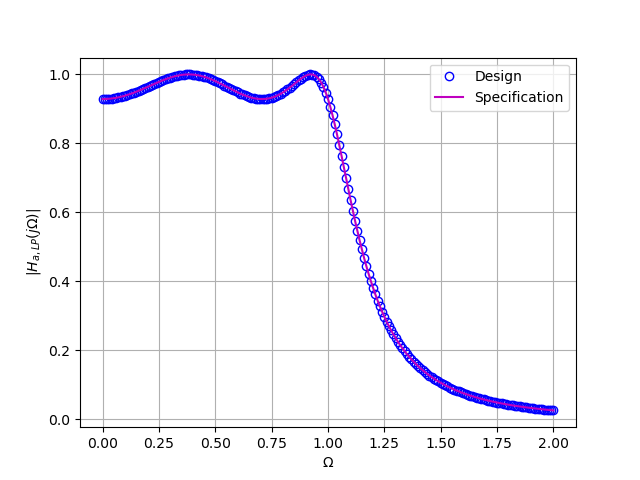
\includegraphics[width =\columnwidth]{fig2.png}
\caption{The magnitude response plots from the specifications in Equation \ref{lpsqfinal} and the design in Equation \ref{lpfinal}}
\label{fig2}
\end{figure}

\begin{figure}[H]
\label{fig3}
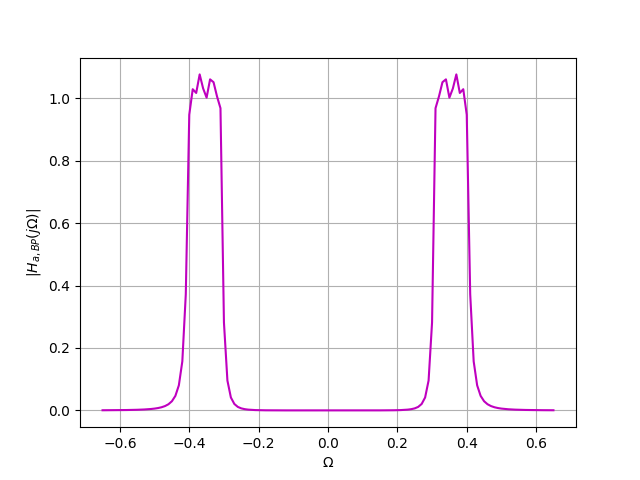
\includegraphics[width = \columnwidth]{fig3.png}
\caption{The analog bandpass magnitude response plot from Equation \ref{bpfinal}} 
\end{figure}

\subsection{The Digital Filter}
From the bilinear transformation, we obtain the digital bandpass filter from the corresponding analog filter as
\begin{eqnarray}
\label{analdig}
H_{d,BP}(z) = GH_{a,BP}(s)\vert_{s = \frac{1-z^{-1}}{1 + z^{-1}}}
\end{eqnarray}
where $G$ is the gain of the digital filter.  From (\ref{bpfinal}) and (\ref{analdig}), we obtain

\begin{eqnarray}
H_{d,BP}(z) = G \frac{N(z)}{D(z)}
\end{eqnarray}
where $G =  2.0601\times 10^{-5}$,

\begin{eqnarray}
N(z)=  1 - 4 z^{-2} + 6 z^{-4} - 4z^{-6} + z^{-8} 
\end{eqnarray}
and
{\small
\begin{eqnarray}
D(z) = 1.7511  -10.6506z^{-1} + 30.9794z^{-2}  -55.1588z^{-3}+  65.4285z^{-4}\nonumber \\
  -52.8121z^{-5}+   28.3995z^{-6}  -9.3484z^{-7} +   1.4717z^{-8}
\end{eqnarray}
}
The plot of $|H_{d,BP}(z)|$ with respect to the normalized angular frequency (normalizing factor $\pi$) is available in Figure 4.  Again we
find that the passband and stopband frequencies meet the specifications well enough.

\begin{figure}[H]
\label{fig4}
\centering
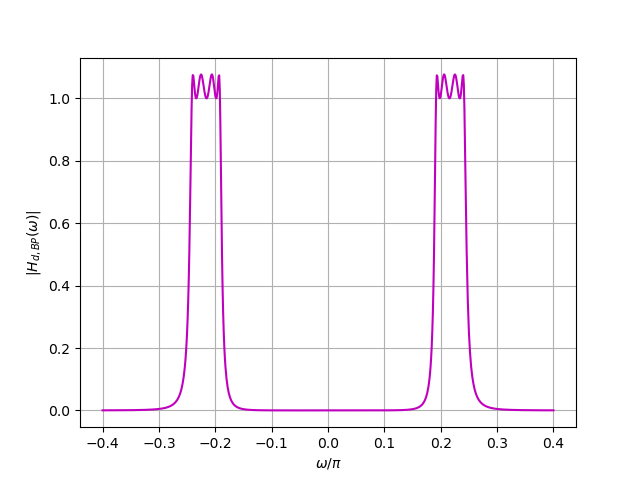
\includegraphics[width = \columnwidth]{fig4.png}
\caption{The magnitude response of the bandpass digital filter designed to meet the given specifications} 
\end{figure}


\section{The FIR Filter}
We design the FIR filter by first obtaining the (non-causal) lowpass equivalent using the Kaiser window
and then
converting it to a causal bandpass filter.

\subsection{The Equivalent Lowpass Filter}
The lowpass filter has a passband frequency $\omega_l$ and transition band $\Delta \omega = 2\pi \frac{\Delta F}{F_s} = 0.0125\pi$.
The stopband tolerance is $\delta$.
\begin{enumerate}
\item  The {\em passband frequency $\omega_l$}  is defined as:
\begin{align}
    \omega_l = \frac{\omega_{p1} - \omega_{p2}}{2}
\end{align}

 Substituting the values of $\omega_{p1}$ and $\omega_{p2}$ from section 2.1, we obtain $\omega_l = 0.025\pi$.

\item {\em The impulse response $h_{lp}(n)$} of the desired lowpass filter with cutoff frequency $\omega_l$
is given by
\begin{eqnarray}
\label{firlpdef}
h_l(n) = \frac{\sin(n\omega_l)}{n\pi}w(n),
\end{eqnarray}
where $w(n)$ is the Kaiser window obtained from the design specifications.
\end{enumerate}

\subsection{The Kaiser Window}
The Kaiser window is defined as
\begin{align}
w(n) =
\begin{cases}
\label{kaiser}
& \frac{I_0\left[ \beta N \sqrt{1 - \left(\frac{n}{N}\right)^2} \right]}{I_0(\beta N)},
\indent -N \leq n \leq N, \indent \beta > 0  \\
& 0 \hspace{2.4cm}\text{otherwise,}
\end{cases}
\end{align}
where $I_0(x)$ is the modified Bessel function of the first kind of order zero in $x$ and $\beta$
and $N$ are the window shaping factors.  In the following,
we find $\beta$ and $N$ using the design parameters in section 2.1.

\begin{enumerate}
\item  N is chosen according to
\begin{equation}
N \geq \frac{A-8}{4.57\Delta \omega},
\end{equation}
where $A = -20\log_{10}\delta$.  Substituting the appropriate values from the design specifications, we obtain
$A = 16.4782$ and $N \geq 48$.

\item  $\beta$ is chosen according to
\begin{eqnarray}
\label{kaisercond}
\beta N = \left\{ \begin{array}{ll} 0.1102(A-8.7) & A > 50 \\
0.5849(A-21)^{0.4}+ 0.07886(A-21) & 21 \leq A \leq 50 \\
0 & A < 21\end{array} \right.
\end{eqnarray}
In our design, we have $A = 16.4782 < 21$.  Hence, from (\ref{kaisercond}) we obtain $\beta = 0$.  

\item We choose $N = 100$, to ensure the desired low pass filter response.  Substituting in (\ref{kaiser})
gives us the rectangular window
\begin{align}
w(n) =
\begin{cases}
& 1, \indent -100 \leq n \leq 100 \\
& 0 \hspace{6mm} \mbox{otherwise}
\end{cases}\label{rect}
\end{align}
\end{enumerate}

From (\ref{firlpdef}) and (\ref{rect}), we obtain the desired lowpass filter impulse response
\begin{align}
h_{lp}(n) =
\begin{cases}
\label{firlpfinal}
& \dfrac{\sin(\frac{n\pi}{40})}{n\pi} \indent -100 \leq n \leq 100  \\
& 0, \hspace{2cm} \mbox{otherwise}
\end{cases}
\end{align}
The magnitude  response of the filter in (\ref{firlpfinal}) is shown in Figure 5.

\begin{figure}[H]
\label{fig5}
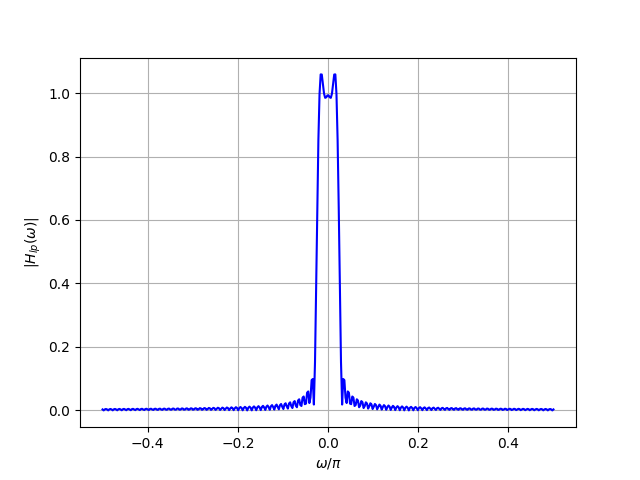
\includegraphics[width = \columnwidth]{fig5.png}
\caption{The magnitude response of the FIR lowpass digital filter designed to meet the given specifications} 
\end{figure}

\subsection{The FIR Bandpass Filter}
The centre of the passband of the desired bandpass filter was found to be $\omega_c = 0.2166\pi$ in Section
2.1.  The impulse response of the desired bandpass filter is obtained from the impulse response of the
corresponding lowpass filter as
\begin{align}
h_{bp}(n) = 2h_{lp}(n)cos(n\omega_c)
\end{align}
Thus, from (\ref{firlpfinal}), we obtain
\begin{align}
h_{bp}(n) =
\begin{cases}
\label{firbpfinal}
& \dfrac{2\sin(\frac{n\pi}{40}) \cos(\frac{13n\pi}{60})}{n\pi} \indent -100 \leq n \leq 100 \nonumber \\
& 0, \hspace{3cm} \mbox{otherwise}
\end{cases}
\end{align}
The magnitude response of the FIR bandpass filter designed to meet the given specifications is plotted in Figure 6.
\begin{figure}[H]
\label{fig6}
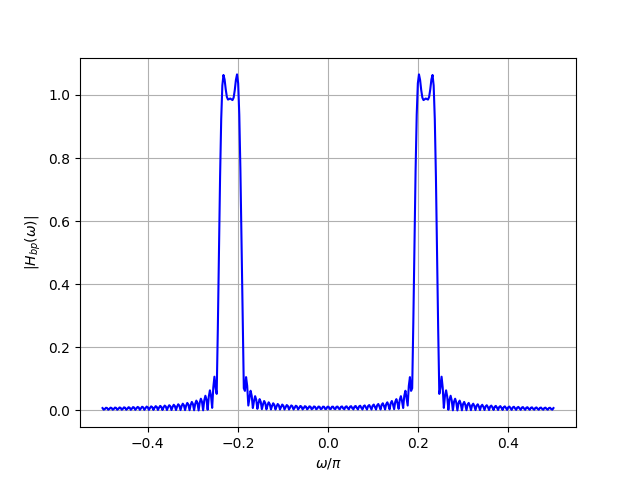
\includegraphics[width = \columnwidth]{fig6.png}
\caption{The magnitude response of the FIR bandpass digital filter designed to meet the given specifications} 
\end{figure}

\end{document}
